\section{Lecture 24: Outlook --- Directions for Analytic Geometry}
\label{lec:24}

This is the final lecture of the course. With Clausen's treatment of Berkovich
spaces (\cref{lec:23}) the programme announced in \cref{lec:1} is complete: the
traditional frameworks of analytic geometry --- complex-analytic, rigid, adic,
Berkovich --- all sit inside analytic stacks, carrying a genuine derived
structure sheaf and a full six-functor formalism. Scholze devotes the last hour
to an \emph{outlook}: a list of directions in which the machinery might be
pushed, ordered from the most developed to the most speculative. The register
is deliberately informal, and much of what follows is flagged by Scholze himself
as conjecture, hope, or a computation he has not carried out; the notes preserve
those hedges.

The personal motivation, restated from the first lecture: for some five or six
years Scholze wanted to do $p$-adic geometry not only $p$-adically but also with
real (archimedean) coefficients and, ideally, in a single framework spanning
both --- and it was always clear that this required a genuinely new language.
That language now exists, and the sensible next question is simply to use it.

Throughout, ``ring'' means commutative ring and everything is (light) condensed.

\subsection{Direction 1: quasi-coherent sheaves and six functors, in all
flavours of analytic geometry}
\label{subsec:24:qcoh}

This first item is not a speculation but something that works. One now has a
general theory of quasi-coherent sheaves --- with no finiteness conditions
imposed on the modules --- in \emph{all} flavours of analytic geometry, and all
those flavours are unified into the single notion of an analytic stack. Better
still, this is a full six-functor formalism
\begin{equation}
\label{eq:24:six-functors}
f^*,\quad f_*,\quad f_!,\quad f^!,\quad \otimes,\quad \RHom ,
\end{equation}
which lets one play. Two immediate payoffs Scholze singled out.

\begin{remark}[A structure sheaf for free]
\label{rmk:24:structure-sheaf}
As Clausen emphasised in \cref{lec:23}, even producing a well-behaved
\emph{structure sheaf} is a nontrivial application. For Berkovich spaces --- even
those of finite type over $\mathbb Z$ --- one classically had to work hard to
define anything; for adic spaces there were the non-sheafiness issues that had
to be resolved by passing to a derived object by hand (\cref{lec:10}). In the
present framework an analytic stack simply comes with its structure sheaf,
period.
\end{remark}

\begin{remark}[GAGA and descent for vector bundles]
\label{rmk:24:gaga-vb}
One can reprove the various GAGA theorems and also prove genuinely new ones
(\cref{lec:15,lec:19,lec:21}). There are also results on descent for vector
bundles. Scholze recalled Drinfeld's work on (infinite-dimensional) vector
bundles \cite{drinfeld2004infinitedimensionalvectorbundlesalgebraic}, where for
the assignment $R\mapsto\{\text{vector bundles on }R(\!(t)\!)\}$ --- something
that arises naturally when thinking about loop groups --- one proves descent
results; a difficult paper, recently revisited by Mathew using his
descendability ideas \cite{mathew2016galoisgroupstablehomotopy}. A further
variant of such Drinfeld-type statements, put to Scholze by a colleague, can be
proved very simply using the general $\RHom$-formulas of the six-functor
formalism.
\end{remark}

Related to Riemann--Roch and to the Atiyah--Singer index theorem (which Scholze
is optimistic could in principle be proved with this technology, though this has
not been figured out): all of these are closely tied to $K$-theory, which is the
next item.

\subsection{Direction 2: \texorpdfstring{$K$}{K}-theory of analytic spaces}
\label{subsec:24:k-theory}

In algebraic geometry, $K$-theory was defined first by Quillen and then for
general schemes by Thomason, using the well-behaved stable $\infty$-category of
perfect complexes. In analytic geometry the obstruction was the absence of a
good enough category of modules to which one could apply categorical
$K$-theoretic techniques. With the present technology one can do it --- not with
perfect complexes exactly, but with a variant of \emph{nuclear} modules
(\cref{def:10:nuclear}). This uses Efimov's $K$-theory of dualizable
$\infty$-categories; the analytic side has been developed in particular by
Andreychev \cite{andreychev2021pseudocoherentperfectcomplexesvector}, who has
worked out the $K$-theory and THH of Tate adic spaces using Efimov's results on
continuous $K$-theory.

\begin{remark}[Localizing motives and refined trace theories]
\label{rmk:24:localizing-motives}
Efimov's strong results on the category of localizing motives (proving it is
rigid, hence dualizable) allow one to define refined variants of cyclic and
topological cyclic homology which do \emph{not} take values in some complete
category: usually, taking $S^1$-fixed points produces a completed power-series
object, whereas here one can instead land in nuclear modules in our sense, tying
these trace theories back into analytic geometry. Clausen mentioned a joint
project bearing on this circle of ideas that would have used nuclear $K$-theory,
though he immediately added that they had since found a way to avoid it.
\end{remark}

\subsection{Direction 3: \texorpdfstring{$p$}{p}-adic cohomology theories}
\label{subsec:24:p-adic}

A great deal of work, much of it already done, concerns $p$-adic coefficient
systems and cohomology theories, where the geometric language of analytic stacks
is directly relevant. Among the incarnations Scholze listed:
\begin{itemize}
\item the \emph{analytic de Rham stack} (Rodr\'iguez Camargo
\cite{camargo2024analyticrhamstackrigid}), which gives a six-functor formalism
for what are essentially $\widehat{\mathcal D}$-modules --- modules over a
completion of the ring of differential operators to differential operators of
infinite order, in the sense of Ardakov--Wadsley --- avoiding the usual
functional-analysis difficulties;
\item the \emph{analytic Hodge--Tate stack} (Anschütz--Heuer--Le Bras);
\item \emph{geometric Sen theory} (Pan, Rodr\'iguez Camargo), with applications
to global automorphic forms, closely related to geometric Langlands;
\item \emph{analytic prismatization};
\item $p$-adic local Langlands for locally analytic representations, phrased in
terms of geometric Langlands on the Fargues--Fontaine curve.
\end{itemize}
Scholze noted Pilloni's recent talk on joint work with Boxer, Calegari and Gee
proving modularity of genus-two curves, whose key technical part uses this kind
of technology, and that one expects a local geometric language for
$p$-adic/locally-analytic representations --- a sheaf-theoretic version of the
Fargues--Scholze geometrization of local Langlands
\cite{fargues2024geometrizationlocallanglandscorrespondence}, and eventually a
global one.

\subsection{Direction 4: the real analogue of the
\texorpdfstring{$p$}{p}-adic coefficient theories}
\label{subsec:24:real}

A focus of the 2023 Hausdorff trimester in Bonn was the realisation that, now
that the $p$-adic story is well understood and phrased in the correct geometric
language, one can more or less translate all of its ingredients to the
\emph{real} world one-to-one. There is a real analogue of virtually everything:
\begin{itemize}
\item a real \emph{analytic de Rham stack}, which in this case is isomorphic to
the \emph{Betti stack} --- the statement of a Riemann--Hilbert correspondence;
\item a real \emph{analytic Hodge stack} (where the relevant gerbe is trivial,
whereas $p$-adically it can be a nontrivial gerbe);
\item an analytic ``prismatization''-type stack whose vector bundles encode, in
the $p$-adic world, variations of Hodge structure; in the real world one gets
\emph{variations of twistor structure}, generalising variations of Hodge
structure (Simpson; Mochizuki's variations of mixed twistor structure), carrying
a $U(1)$-action;
\item and, synthesising these, a \emph{real local Langlands} for locally
analytic representations of $G(\mathbb R)$, phrased as geometric Langlands on the
\emph{twistor-$\mathbb P^1$} (the real analogue of the Fargues--Fontaine curve).
Here the classical Harish-Chandra $(\mathfrak g,K)$-modules are replaced by a
genuinely geometric object: the derived category of the classifying stack of the
real-locally-analytic group, together with its forgetful functor to
$\mathbb C_{\gasx}$-modules,
\begin{equation}
\label{eq:24:real-langlands}
D\bigl(\operatorname{Spec}\mathbb C_{\gasx}\,/\,G(\mathbb R)^{R\text{-}\mathrm{la}}\bigr)\ \longrightarrow\ D(\mathbb C_{\gasx}).
\end{equation}
\end{itemize}

\begin{remark}[Representations of $G(\mathbb R)$ without Harish-Chandra modules]
\label{rmk:24:real-reps}
Usually, representations of $G(\mathbb R)$ force functional-analysis issues, and
one replaces them by the more algebraic Harish-Chandra
$(\mathfrak g,K)$-modules --- passing to $K$-finite vectors for a maximal compact
$K$ --- at the cost of collapsing many representations (with different function
spaces but the same Harish-Chandra module) to one. In the present world one can
encode representations of the real group directly and need not do this. Concretely,
$G(\mathbb R)$ is a group object in real-analytic manifolds, so its
real-analytic incarnation is a group object in analytic stacks; one forms the
classifying stack $BG(\mathbb R)$ (over $\mathbb C_{\gasx}$, say), whose
quasi-coherent sheaves are representations of the group. To realise them as
representations one pulls back along the projection $\pi$ from a point: for a
canonical object attached to a Harish-Chandra module, $\pi^*$ should produce the
minimal globalisation and $\pi^!$ the maximal globalisation (this has not yet
been checked). This is closely related to the existence of enough analytic
vectors in representations.
\end{remark}

\subsection{Direction 5: metrics and the extended Berkovich line}
\label{subsec:24:metrics}

Here we enter the speculative realm, though with a strong belief. Classically, in
questions of functoriality and in geometry, one often has to put \emph{metrics}
on things --- to prove a Hodge decomposition, say, one does $L^2$-analysis. We
cannot yet translate anything involving metrics into our world. Scholze's guess
for where they should enter is the \emph{extended} Berkovich line of $\mathbb Z$
from \cref{lec:22} (\cref{thm:22:image}, \cref{fig:22:MZ}): the Berkovich tree
with its central trivial-norm point, one branch per prime $p$ ending at
$\mathbb F_p$, and the archimedean branch --- but where the classical Berkovich
space stops the archimedean branch at $|\cdot|_\infty$ (because of the triangle
inequality), our space of norms imposes no triangle inequality, so the
archimedean branch is prolonged past $|\cdot|_\infty$ and then one-point
compactified, adding a point at infinity. The intuition is that
\emph{this point at infinity must be related to metrics.}

\begin{remark}[Evidence from the $p$-adic side]
\label{rmk:24:metric-evidence}
Working $2$-adically, extending over the endpoint $\mathbb F_2$ of the
$2$-branch means precisely putting a $\mathbb Z_2$-module over $\mathbb Z_2$
above the generic $\mathbb Q_2$-vector space --- i.e.\ a $2$-adic
\emph{integral} structure, a $p$-adic metric. So by analogy, extending over the
archimedean point at infinity ought to mean putting some kind of metric on real
objects.
\end{remark}

The analogy between $p$ and $\infty$ can be made sharper. Over the open part of a
$p$-branch one has a $p$-adic locally analytic space
\begin{equation}
\label{eq:24:qp-la}
\mathbb Q_p^{\mathrm{la}}\ =\ \bigcup_{n} p^{-n}\,\mathbb Z_p^{\mathrm{la}},
\qquad
\mathbb Z_p^{\mathrm{la}}\ =\ \AnSpec\, C^{\mathrm{la}}(\mathbb Z_p,\mathbb Q_p),
\end{equation}
where $C^{\mathrm{la}}(\mathbb Z_p,\mathbb Q_p)$ are the locally analytic
functions --- those locally developable into a power-series expansion. Since it
has $\mathbb Q_p$-coefficients, this space, which lives over the open $p$-adic
ray, has a canonical extension over the endpoint $\mathbb F_p$; this is closely
related to a theory of locally analytic representations of $G(\mathbb Q_p)$. The
canonical extension is somewhat subtle to write down but its existence matters
for the $p$-adic story.

The real analogue: over the open archimedean ray one has the real-analytic
$\mathbb R$, i.e.\ $\mathbb R$ as a real-analytic manifold with functions the
real-analytic functions (again, locally power-series expansions), each fibre over
a point of the ray being a copy of $\mathbb R^{\mathrm{an}}$. Scholze conjectures
this extends canonically over the closed point at infinity, and likewise that the
real-analytic group $G(\mathbb R)^{\mathrm{an}}$ extends canonically over that
point. (One uses the gaseous structure at all points; the liquid structure is not
needed here.) At every point of the ray there is a rescaling action of the norm,
so a whole family of copies of the reals, mapping to the space of norms as an open
subspace.

\begin{remark}[Geometry over the point at infinity]
\label{rmk:24:geometry-at-infinity}
More broadly, one can look at analytic stacks over the space of norms that map to
the closed point at infinity, and ask what geometry lives there. It is a very
peculiar geometry --- still about real/complex manifolds, but where one can
localise much more, zooming in infinitesimally. For instance, on the Riemann
sphere the ``bounded'' part is not quite the closed unit disc but some minimally
overconvergent neighbourhood of it: essentially the closed unit disc, but any
real number bigger than $1$ is an unbounded function on it. Scholze expects that
whatever geometry lives over this point is exactly what is needed to prove
statements (like the Hodge decomposition for complex projective manifolds) that
classically require putting metrics on things; this remains to be understood.
\end{remark}

\subsection{Direction 6: sheaves of higher categories, and quantum
Chern--Simons}
\label{subsec:24:higher-cats}

Our formalism removes the classical obstruction of having to do functional
analysis and fancy category theory at the same time; once that is gone, one can
go completely fancy. To an affine analytic space one first associates its derived
category $D(A)$, then the module category $\PrL_{D(A)}=\Mod_{D(A)}(\PrL)$; but
one can iterate, using Stefanich's presentable $(\infty,n)$-categories
$n\PrL$ for any $n$,
\begin{equation}
\label{eq:24:nprl}
A\ \longmapsto\ D(A),\quad \PrL_{D(A)},\quad 2\PrL_{D(A)},\quad \dots,\quad
n\PrL_X ,
\end{equation}
defining $n\PrL_X$ for any stack $X$, again with a six-functor formalism to play
with. The existence of this is not speculative; what follows is.

The speculation is a construction of \emph{quantum Chern--Simons theory} via the
cobordism hypothesis. Let $G$ be a compact, simple, simply connected Lie group,
so that the first interesting cohomology is $H^3(G,\mathbb Z)\cong\mathbb Z$; fix
a level
\begin{equation}
\label{eq:24:level}
\ell\ \in\ H^3(G,\mathbb Z).
\end{equation}
Regarding $\ell$ as a map $G\to B^3\mathbb Z$ of groups, it deloops to a map
$BG\to B^4\mathbb Z$, i.e.\ a class in $H^4(BG,\mathbb Z)=\mathbb Z$. Now restrict
to the real-analytic incarnation $BG^{\mathrm{an}}$ (using that any real-analytic
manifold $M$ maps to its condensed incarnation $M^{\mathrm{cond}}$). Using the
exponential sequence
\begin{equation}
\label{eq:24:exponential}
0\ \longrightarrow\ 2\pi i\,\mathbb Z\ \longrightarrow\ \mathbb G_a\
\xrightarrow{\ \exp\ }\ \mathbb G_m\ \longrightarrow\ 0 ,
\end{equation}
the composite $BG^{\mathrm{an}}\to B^4\mathbb Z\to B^4\mathbb G_a$ vanishes ---
this is coherent cohomology, and it is here that compactness of $G$ is crucial
--- so the level lifts to a map
\begin{equation}
\label{eq:24:alpha}
\alpha\colon\ BG^{\mathrm{an}}\ \longrightarrow\ B^3\mathbb G_m ,
\end{equation}
as in the lifting triangle

% Provenance: board 13 (00:52:52) --- the level, its delooping, and the lift to
% B^3 G_m through the exponential sequence 0 -> 2 pi i Z -> G_a -> G_m -> 0.
\begin{equation}
\label{eq:24:lift-diagram}
\begin{tikzcd}[column sep=large, row sep=large]
& B^3\mathbb G_m \arrow[d] \\
BG^{\mathrm{an}} \arrow[ur, "\alpha", dashed]
  \arrow[r, "\ell"'] & B^4\mathbb Z \arrow[r] & B^4\mathbb G_a
\end{tikzcd}
\end{equation}
with the bottom composite zero.

A map to $B\mathbb G_m$ is a line bundle; a map to $B^2\mathbb G_m$ gives a twist
of the category of modules; a map to $B^3\mathbb G_m$ gives a twist of the
category of \emph{categories}, i.e.\ $\alpha$ specifies an invertible object
$L\in 2\PrL_{BG^{\mathrm{an}}}$. One then pushes forward along the projection
$\pi\colon BG^{\mathrm{an}}\to\ast$ (with $\ast=\operatorname{Spec}\mathbb C_{\gasx}$), forming
--- morally the space of conformal blocks ---
\begin{equation}
\label{eq:24:conformal-blocks}
\pi_!\,\alpha^*L\ \in\ 2\PrL_{\mathbb C_{\gasx}} .
\end{equation}
(For $G$ a finite group this is literally an integral over the space of
$G$-bundles, the situation of Freed--Hopkins--Lurie--Teleman
\cite{freed2009topologicalquantumfieldtheories}.)

\begin{remark}[Is it $3$-dualizable?]
\label{rmk:24:dualizable}
A three-dimensional topological field theory should, by the cobordism
hypothesis, be a $3$-dualizable object of a $3$-category, and $2\PrL$ furnishes
one. So: is \eqref{eq:24:conformal-blocks} $3$-dualizable? An expert would say
immediately there is no chance, because a holomorphicity constraint (the space of
conformal blocks) is missing. But one is not far off: Scholze believes it is
$2$-dualizable, and $3$-dualizability would require, for
$\pi\colon BG^{\mathrm{an}}\to\ast$ and its iterated diagonals, that
\begin{equation}
\label{eq:24:six-conditions}
\pi,\quad \Delta_\pi,\quad \Delta_{\Delta_\pi}
\quad\text{each be proper and smooth} ,
\end{equation}
six conditions in all. Only one fails: the \emph{smoothness of $\pi$} (of
$G^{\mathrm{an}}$ itself). The obstruction is exactly coherent cohomology --- for
the condensed-set classifying stack, coherent cohomology is singular cohomology,
so had one used $B^4\mathbb G_a$ over the complex numbers ($BG_{\mathbb C}$) the
lift would have failed on $H^4(BG;\mathbb C)$; it is the compact/real-analytic
structure that makes the relevant cohomology vanish. Scholze's hope is that
tweaking the construction --- e.g.\ replacing $\mathbb R^{\mathrm{an}}$ by the
canonical extension over the point at infinity of Direction 5, or incorporating
the connection / Deligne-cohomology (weight-two) structure that the map to
$B^3\mathbb G_m$ really carries --- supplies the missing holomorphicity
constraint. The point is that one can now just \emph{play} with these objects
naively, where classically one would drown in functional analysis.
\end{remark}

\begin{remark}[The exponential sequence as a sequence of stacks]
\label{rmk:24:exponential-stacks}
Asked in what sense \eqref{eq:24:exponential} is exact: all of $2\pi i\,\mathbb Z$,
$\mathbb G_a^{\mathrm{an}}$, $\mathbb G_m^{\mathrm{an}}$ are analytic stacks with a
commutative group structure --- sheaves of abelian-group objects in the higher
(anima) sense --- and \eqref{eq:24:exponential} is an exact sequence of these,
connected and also surjective on the right. It is not stable, but passing to the
$B$-groups puts it in a stable context.
\end{remark}

\subsection{Direction 7: virtual fundamental classes}
\label{subsec:24:vfc}

The last direction is treated in more detail; after the very fancy Direction 6 it
is comparatively concrete. It concerns a theory of \emph{virtual fundamental
classes}. Such classes arise, for instance, in symplectic geometry (Gromov--Witten
invariants). In algebraic situations there has been a known solution for some
twenty or thirty years, but the genuinely analytic context is much more subtle,
and it is exactly the kind of setting --- objects that are simultaneously
analytic, derived and stacky --- where our theory should be useful. Scholze
reports that it can indeed do something.

\begin{question}[Signed intersection count]
\label{q:24:signed-count}
Consider a fibre product of oriented compact smooth manifolds

% Provenance: board 14 (01:00:19) --- the model fibre-product square.
\begin{equation}
\label{eq:24:fibre-product}
\begin{tikzcd}[column sep=large, row sep=large]
X \arrow[r] \arrow[d] & M_1 \arrow[d] \\
M_2 \arrow[r] & M
\end{tikzcd}
\end{equation}
(one may assume $M_1,M_2\hookrightarrow M$ are closed immersions), of
\emph{expected dimension $0$}:
\begin{equation}
\label{eq:24:expected-dim-zero}
\dim M_1+\dim M_2\ =\ \dim M .
\end{equation}
If the intersection is transverse, $X$ is a finite oriented set of points, so one
has a well-defined signed count
\begin{equation}
\label{eq:24:signed-count}
\#^{\mathrm{sgn}}(X)\ \in\ \mathbb Z ,
\end{equation}
invariant under perturbations (as long as the intersection stays transverse).
Can one define $\#^{\mathrm{sgn}}(X)$ in general --- without transversality or
perturbation --- purely intrinsically on $X$?
\end{question}

Each connected component ought to carry a well-defined local contribution (as in
Fulton's intersection theory), but even the local numbers must be defined. The
difficulty is that for smooth manifolds the intersection, as a topological space,
has essentially no structure: two curves in a surface can be tangent to infinite
order, agree along an interval and then separate, accumulate infinitely many
components, and so on. (For smooth projective varieties the intersection cannot be
so wild, and there the problem is classical.)

\begin{theorem}[Virtual fundamental classes exist]
\label{thm:24:vfc-exists}
Yes: provided the fibre product \eqref{eq:24:fibre-product} is computed in our
category --- so that $X$ is a \emph{derived} smooth manifold --- and, crucially,
worked over the \emph{liquid} real numbers $\mathbb R^{\mathrm{liq}}$ (for some
choice of the liquid parameter, which does not affect the outcome) rather than the
gaseous reals. One can define the class of analytic stacks that are locally such
an intersection, and construct a virtual fundamental class on them.
\end{theorem}

The liquid structure --- irrelevant for essentially everything else in the course
--- is genuinely used here (\cref{rmk:24:liquid-tensor} below). Symplectic experts
at MPI (Nate Botman, Katrin Wehrheim) pointed out that even the simplest case is
surprising; the following explains why.

\subsubsection*{The surprising local computation}

Take $M_1,M_2$ two curves in a surface meeting locally at a single point, and
analyse a neighbourhood via the vanishing of a function.
\begin{itemize}
\item Transverse $\Rightarrow$ a point, counting $\pm1$.
\item Quadratic tangency $\Rightarrow 0$; cubic $\Rightarrow \pm1$; and in general,
if the function vanishes to \emph{finite} order one simply remembers the vanishing
order, which decides whether the graph crosses the line.
\end{itemize}
The subtle case is infinite-order tangency. Consider the two functions
\begin{equation}
\label{eq:24:two-functions}
e^{-1/x^2}\qquad\text{and}\qquad \operatorname{sgn}(x)\,e^{-1/x^2},
\end{equation}
both vanishing to infinite order at $0$; the first stays positive (does not cross
the axis), the second crosses.

% Provenance: board 16 (01:06:16) --- the two graphs (infinite-order tangency vs.
% crossing); redrawn schematically. Board exponent read as -1/x^2.
\begin{figure}[ht]
\centering
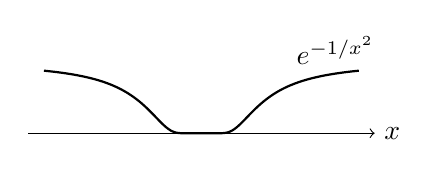
\begin{tikzpicture}[scale=1.0]
  \draw[->] (-2.2,0) -- (2.2,0) node[right] {$x$};
  % e^{-1/x^2}: positive bump touching axis at 0, does not cross
  \draw[thick,domain=-2:2,samples=120,smooth,variable=\x]
    plot ({\x},{0.9*exp(-0.5/(\x*\x+0.001))});
  \node at (1.7,1.05) {$e^{-1/x^2}$};
\end{tikzpicture}\qquad
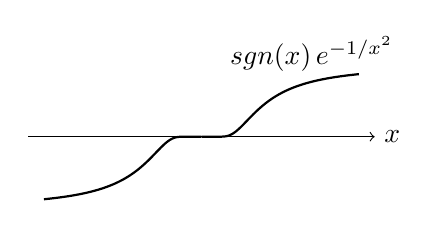
\begin{tikzpicture}[scale=1.0]
  \draw[->] (-2.2,0) -- (2.2,0) node[right] {$x$};
  % sgn(x) e^{-1/x^2}: crosses the axis at 0
  \draw[thick,domain=0.001:2,samples=80,smooth,variable=\x]
    plot ({\x},{0.9*exp(-0.5/(\x*\x+0.001))});
  \draw[thick,domain=-2:-0.001,samples=80,smooth,variable=\x]
    plot ({\x},{-0.9*exp(-0.5/(\x*\x+0.001))});
  \node at (1.4,1.05) {$\operatorname{sgn}(x)\,e^{-1/x^2}$};
\end{tikzpicture}
\caption{Two functions with the same vanishing locus $\{0\}$ set-theoretically:
$e^{-1/x^2}$ touches the axis without crossing, $\operatorname{sgn}(x)\,e^{-1/x^2}$
crosses. As liquid analytic rings their vanishing loci differ, and that difference
detects the crossing.}
\label{fig:24:two-functions}
\end{figure}

\noindent The claim is that the \emph{vanishing locus} of such a function
distinguishes these two cases --- in particular, determines whether the graph
crosses the line --- in every category. Classically it is unclear what structure
the intersection point should carry: it must remember more than all the
derivatives of the function (which it cannot double), yet much less than the full
germ. In our world it knows exactly the right amount.

\begin{definition}[Vanishing locus]
\label{def:24:vanishing-locus}
For $f\in C^\infty(\mathbb R,\mathbb R)$ with an isolated zero at $0$, the
\emph{vanishing locus} is
\begin{equation}
\label{eq:24:vanishing-locus}
\AnSpec\, C^\infty(\mathbb R,\mathbb R)/(f).
\end{equation}
If $f$ vanishes to order $n$ this is the truncated polynomial $\mathbb R$-algebra
$\mathbb R[T]/T^n$; if $f$ vanishes to infinite order it is a non-Hausdorff
$\mathbb R$-algebra. In the latter case $f$ is still a non-zero-divisor, so
$C^\infty(\mathbb R,\mathbb R)/(f)$ is concentrated in degree $0$ --- only
non-separated, which is exactly what the condensed/liquid framework handles.
\end{definition}

\begin{proposition}[The vanishing locus determines $f$ up to a unit]
\label{prop:24:vanishing-unit}
Let $f,g\in C^\infty(\mathbb R,\mathbb R)$ be as in
\cref{def:24:vanishing-locus}, and suppose there is an isomorphism of condensed
$\mathbb R$-algebras
\begin{equation}
\label{eq:24:iso-quotients}
C^\infty(\mathbb R,\mathbb R)/(f)\ \cong\ C^\infty(\mathbb R,\mathbb R)/(g).
\end{equation}
Then $f=g\cdot u$ for a unit $u\in C^\infty(\mathbb R,\mathbb R)^\times$. In
particular $f$ crosses the line if and only if $g$ does, since an invertible
smooth function $\mathbb R\to\mathbb R$ is everywhere positive or everywhere
negative and multiplying by it cannot change the crossing.
\end{proposition}

\begin{remark}[What the isomorphism must respect]
\label{rmk:24:iso-coordinate}
The isomorphism \eqref{eq:24:iso-quotients} should be one of condensed
$\mathbb R$-algebras carrying the coordinate; only the isolated zero at $0$ is
used. The statement is genuinely surprising: functions of visibly different
decay rate at $0$, such as $e^{-1/x^2}$ and $e^{-1/(cx)^2}$, do have isomorphic
vanishing loci (after a reparametrisation), even though the isomorphism of
abstract condensed algebras looks as if it should see different coordinates. It
is nonetheless true.
\end{remark}

\begin{proof}[Proof of \cref{prop:24:vanishing-unit}]
The engine is the liquid tensor computation (\cref{rmk:24:liquid-tensor}): for
$f,g$ as above one shows that $C^\infty(\mathbb R,\mathbb R)$ is an
\emph{idempotent} algebra over $\mathbb R[T]$ ($T$ the coordinate). Both
$A:=C^\infty(\mathbb R,\mathbb R)/(f)$ and $B:=C^\infty(\mathbb R,\mathbb R)/(g)$
carry a unique evaluation map to $\mathbb R$ (maps $C^\infty(\mathbb R,\mathbb R)\to
\mathbb R$ are classified by real numbers, and only the one at $0$ descends to the
quotient); these commute with the isomorphism. Now given the map
$\mathbb R[T]\to B$, one checks that it extends (necessarily uniquely, by
idempotency of $C^\infty(\mathbb R,\mathbb R)$ over $\mathbb R[T]$) to
$C^\infty(\mathbb R,\mathbb R)\to B$: existence is seen by classifying maps
$\mathbb R[T]\to C^\infty(\mathbb R,\mathbb R)$, which are given by smooth
functions $\mathbb R\to\mathbb R$ and along which any further smooth function may
be composed. Hence the isomorphism upgrades to one respecting the
$C^\infty(\mathbb R,\mathbb R)$-structure, the two presentations of the ideal
agree, and $f=g\cdot u$ up to a reparametrisation.
\end{proof}

\begin{remark}[Liquid, not gaseous]
\label{rmk:24:liquid-tensor}
Working over $\mathbb R^{\mathrm{liq}}$ is essential. The liquid tensor product
computes the expected thing on nuclear Fréchet spaces (spelled out in the
complex-geometry notes \cite{clausen2020analytic}), so that
\begin{equation}
\label{eq:24:liquid-tensor}
C^\infty(M_1)\ \otimes_{\mathbb R^{\mathrm{liq}}}^{\mathbb L}\ C^\infty(M_2)\
\cong\ C^\infty(M_1\times M_2),
\end{equation}
whereas over $\mathbb R_{\gasx}$ one would get a strictly smaller ring. The liquid
building blocks are essentially the $\alpha$-locally-convex ones with $\alpha$
slightly below $1$, so forming these tensor products allows all (nearly)
locally-convex combinations; with nuclear transition maps the precise summability
parameter does not matter. From \eqref{eq:24:liquid-tensor} one deduces the
idempotence of $C^\infty(\mathbb R,\mathbb R)$ over $\mathbb R[T]$ used above.
\end{remark}

\begin{remark}[A $C^\infty$-ring structure for free]
\label{rmk:24:cinfty-ring}
Existing theories of derived (or ``$C^\infty$-'') manifolds build in, by
definition, the datum that any function can be composed with an arbitrary smooth
function $\mathbb R\to\mathbb R$. The observation above shows that our funny
derived vanishing loci \emph{acquire} this structure canonically --- whenever one
has a function, it extends uniquely to compose with smooth functions --- so it
need not be imposed at the outset. This is precisely what makes the objects
comparable.
\end{remark}

\subsubsection*{The general theorem and construction}

\begin{theorem}[Virtual fundamental class]
\label{thm:24:vfc}
Let $S$ be a locally compact Hausdorff, finite-dimensional space equipped with a
sheaf $\mathcal O_S$ of animated liquid $\mathbb R$-algebras, such that
$(S,\mathcal O_S)$ is locally the (smooth, geometric) intersection of smooth
manifolds. Then one can define an \emph{expected dimension}
$d\in H^0(S,\mathbb Z)$, an \emph{orientation sheaf} $\omega_S$ (a
$\mathbb Z$-local system), and a virtual fundamental class
\begin{equation}
\label{eq:24:vfc-class}
\vfc(S,\mathcal O_S)\ \in\ H^0\!\bigl(S,\ \pi^!\mathbb Z\otimes\omega_S[-d]\bigr),
\qquad \pi\colon S\to\ast .
\end{equation}
In particular, if $d=0$, $S$ is compact and an orientation is chosen, one obtains
the signed count
\begin{equation}
\label{eq:24:global-count}
\#^{\mathrm{sgn}}(S,\mathcal O_S)\ =\ \int_S\vfc(S,\mathcal O_S)\ \in\ \mathbb Z ,
\end{equation}
the integral being the trace $\pi_!\pi^!\mathbb Z\to\mathbb Z$ available for
compact $S$.
\end{theorem}

The construction is the direct analogue of the algebro-geometric one (Behrend--%
Fantechi \cite{behrend1996intrinsicnormalcone}, and later many others including
Khan), built on the \emph{intrinsic normal cone}.

\begin{remark}[The intrinsic normal cone]
\label{rmk:24:intrinsic-cone}
Over $S$ there is an intrinsic normal cone $\mathfrak C_S\to S$ whose fibres are a
geometric incarnation of the cotangent complex $L_{\mathcal O_S/\mathbb R}$. For a
derived intersection of smooth things this cotangent complex is perfect of
amplitude $[0,1]$, so the cone needs only $1$-truncated (group-like) directions:
tangent directions give stacky directions, and the obstruction (non-smooth) part
gives vector-bundle directions. Its rank difference is the expected dimension $d$,
and the same geometry produces the orientation sheaf $\omega_S$.
\end{remark}

Concretely, for a compact Hausdorff (or profinite) test object $T$,
\begin{equation}
\label{eq:24:cone-points}
\Homop(T,S)=\Maps\bigl(\AnSpec C(T,\mathbb R),\AnSpec(S,\mathcal O_S)\bigr),
\end{equation}
which is just maps $T\to$ (underlying set), while maps into the intrinsic normal
cone are
\begin{equation}
\label{eq:24:cone-points-cone}
\Homop(T,\mathfrak C_S)=\Maps\bigl(\AnSpec\bigl(C(T,\mathbb R)\otimes_{\mathbb R}
\mathbb R[\epsilon]\bigr),\AnSpec(S,\mathcal O_S)\bigr),
\qquad |\epsilon|=1,\ \epsilon^2=0
\end{equation}
--- i.e.\ one takes the source and mods out $0$ in the derived sense, adjoining
$\epsilon$ in homological degree $1$. Deformation theory then reads off the fibres
as the geometric incarnation of the dual of the cotangent complex.

To extract a class one uses a deformation-to-the-cone picture. Over $\mathbb R$ one
writes a cone $\operatorname{Cone}(S)$ which everywhere except at $0$ is just a
point (the tautological section), but which degenerates, over $0$, to the sticky
intrinsic normal cone $\mathfrak C_S$: on $T$-points, a map corresponds to
$g\in C(T,\mathbb R)$ together with a lift over
$C(T,\mathbb R)\otimes_{\mathbb R}\bigl(C^\infty(\mathbb R,\mathbb R)/(g)\bigr)$,
so that $g=0$ recovers $\mathfrak C_S$, $g$ invertible gives a point, and $g$
somewhere-zero glues the two. One then forms
\begin{equation}
\label{eq:24:cone-sheaf}
F\ :=\ \pi_{\mathrm{cone}\,*}\,\pi_{\mathrm{cone}}^{!}\,\mathbb Z
\end{equation}
and, with $j$ the open inclusion of the cone away from $0$ and $i$ the closed
inclusion of the fibre over $0$, the excision triangle
\begin{equation}
\label{eq:24:excision}
j_!\,j^*F\ \longrightarrow\ F\ \longrightarrow\ i_*\,i^*F
\end{equation}
produces a boundary map. Generically $F$ has a canonical section (the point);
degenerating that section over the special fibre, and accounting for the fibre
bundle by which the cone differs from $S$ (which supplies both the dimension shift
and the orientation sheaf), the boundary map lands the tautological class of
$H^0(\mathbb R\smallsetminus\{0\},\mathbb Z)$ --- taken to be $0$ on one component
and $1$ on the other, with a shift by $\pm1$ because $\mathbb Z$ is taken on the
real line rather than pulled back from a point --- into the desired
$\vfc(S,\mathcal O_S)$.

\begin{remark}[The cone is only shriekable, not smooth]
\label{rmk:24:cone-shriekable}
The map $\pi_{\mathrm{cone}}$ is \emph{not} cohomologically smooth --- the base
$S$ is completely nasty in general, and the cone is some fibrewise
vector-bundle-like object over it, with no reason to be smooth --- but it is
shriekable, which is all one needs to degenerate the tautological fundamental
class and read off the virtual class. The whole construction needs only that the
relevant map be shriekable; the transversal-manifold case guarantees this and it
is stable under fibre products.
\end{remark}

\begin{remark}[Closing]
\label{rmk:24:closing}
Botman asked whether the sticky degeneration here is the same phenomenon as the
compactification over the point at infinity of Direction 5; Scholze did not see
the connection and left it open. This concluded the course.
\end{remark}
